\section{Бегущий огонек}
\begin{verbatim}
	Начальное состояние: вкл
	Движение: Туда/обратно c 10
	Порядок: 9-8-7-6-5-4-3-2-1-0-1-2-3-4-5-6-7-8
\end{verbatim}
\begin{figure}[H]
	\centering
	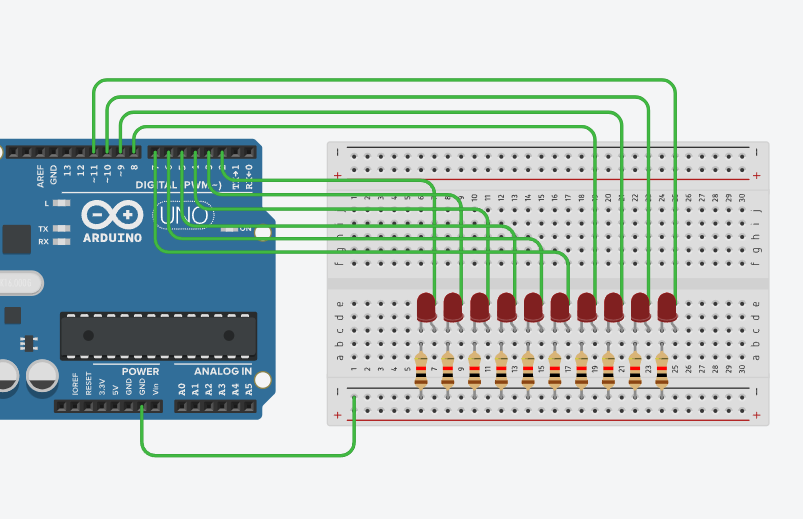
\includegraphics[width=17cm]{z1/1.png}
	\caption{схема сборки}
\end{figure}
\begin{figure}[H]
	\centering
	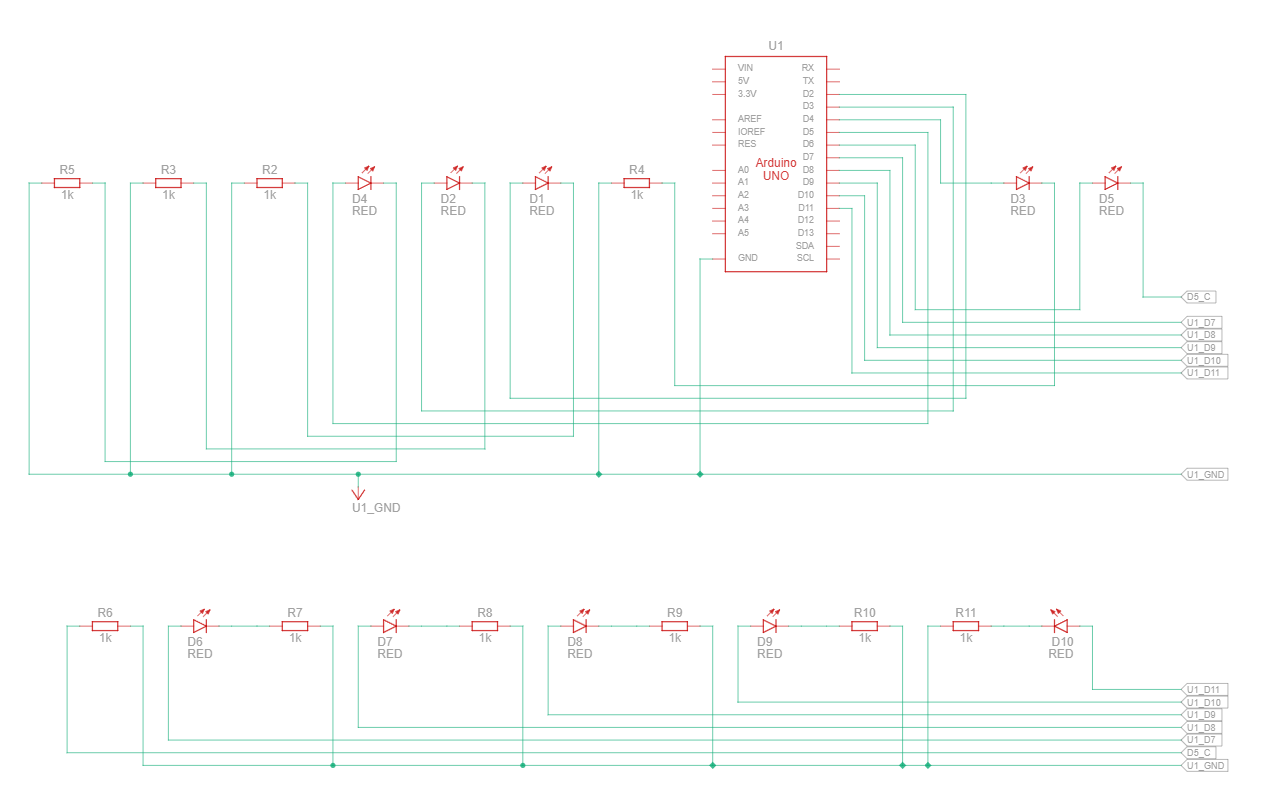
\includegraphics[width=17cm]{z1/2.png}
	\caption{принципиальная схема}
\end{figure}
Код прошивки:
\inputminted{cpp}{z1/main.cpp}
Код поочередно зажигает и гасит 10 светодиодов с задержкой 120 мс, вычисляя номер активного пина с помощью счетчика шагов и переменной направления. При достижении крайнего правого или левого светодиода направление движения инвертируется, заставляя «огонек» бежать обратно.

\section{Пульсар}
\begin{verbatim}
	Начальное состояние: вкл
	Транзистор: биполярный
	Смена состояний: уменьшение до середны/сброс/уменьшение min
\end{verbatim}
\begin{figure}[H]
	\centering
	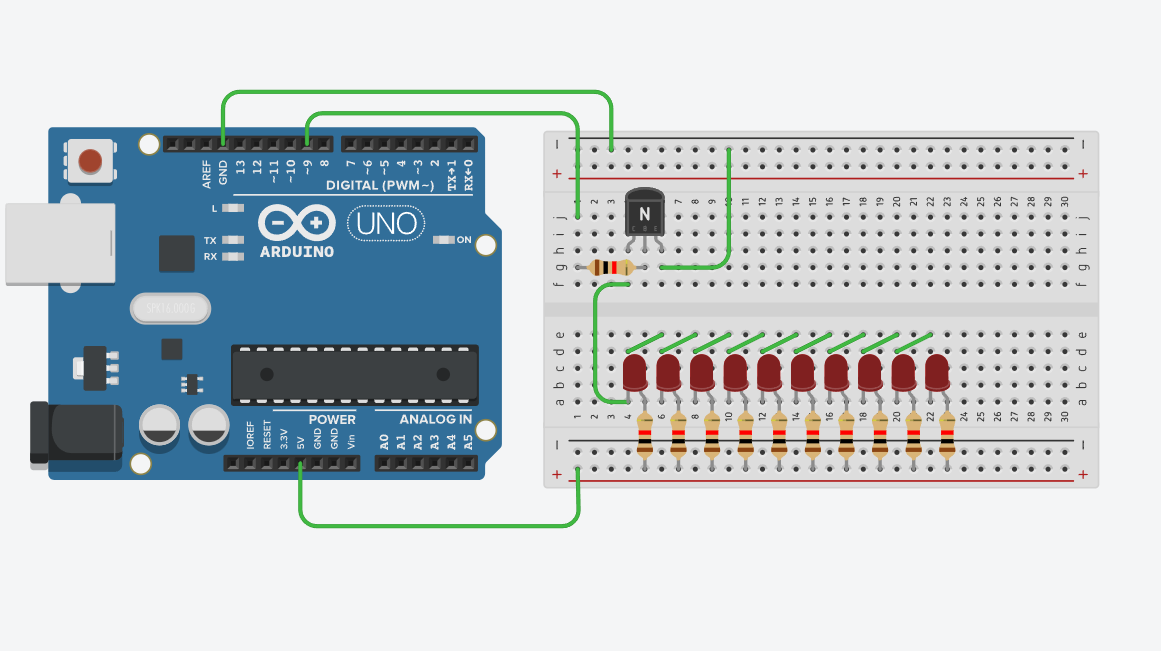
\includegraphics[width=17cm]{z2/1.png}
	\caption{схема сборки}
\end{figure}
\begin{figure}[H]
	\centering
	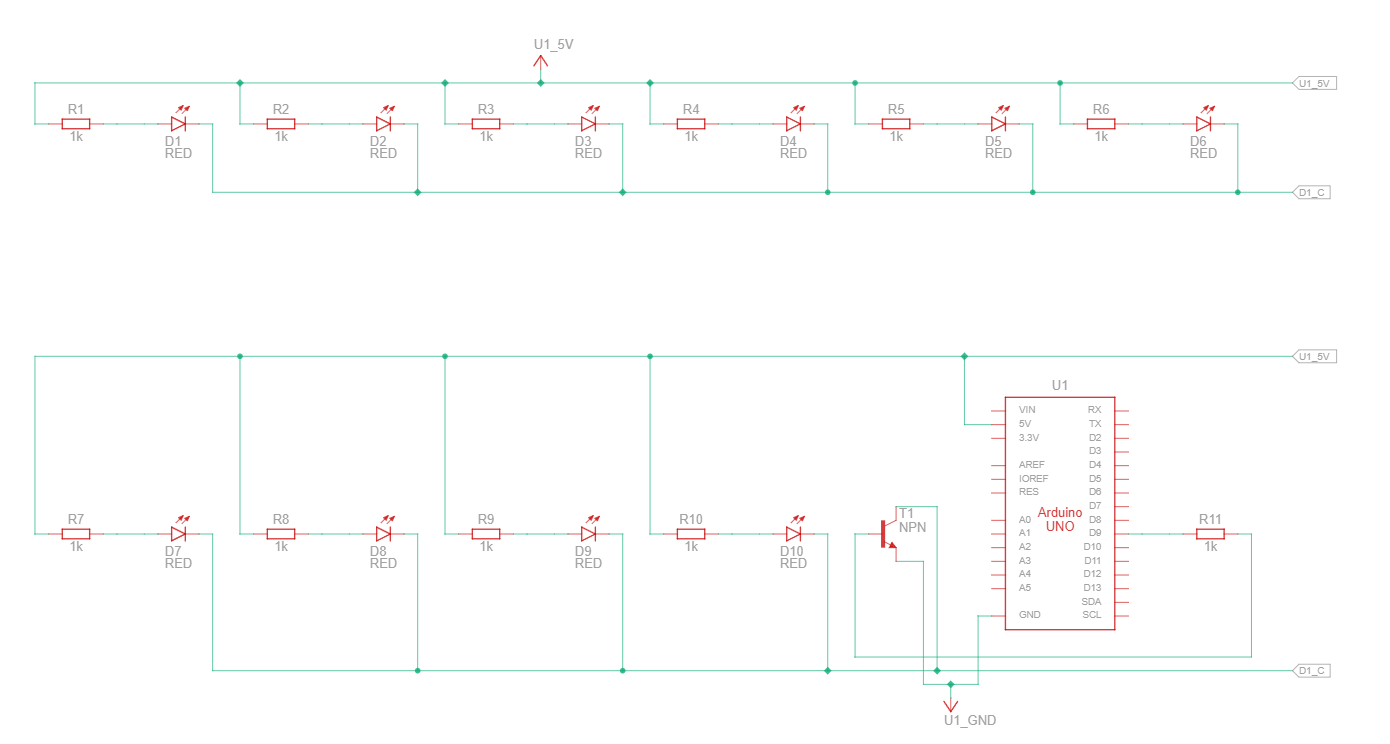
\includegraphics[width=17cm]{z2/2.png}
	\caption{принципиальная схема}
\end{figure}
Код прошивки:
\inputminted{cpp}{z2/main.cpp}
Значение яркости постоянно уменьшается, когда доходит до значения 255/2*k или 0 - сбрасывается до максимума, а также изменяется значение счетчика-множителя k, от которого зависит порог понижения яркости.
https://www.tinkercad.com/things/a8b9i4gsNPk-prak-1-2-pulsar
\section{Ночной светильник}
\begin{verbatim}
	Начальное состояние: выкл
	Входной сигнал: фоторезистор
	Делитель напряжения: 100 кОм
	Смена состояний: Увеличение в зависимости
	от значения на датчике
\end{verbatim}
\begin{figure}[H]
	\centering
	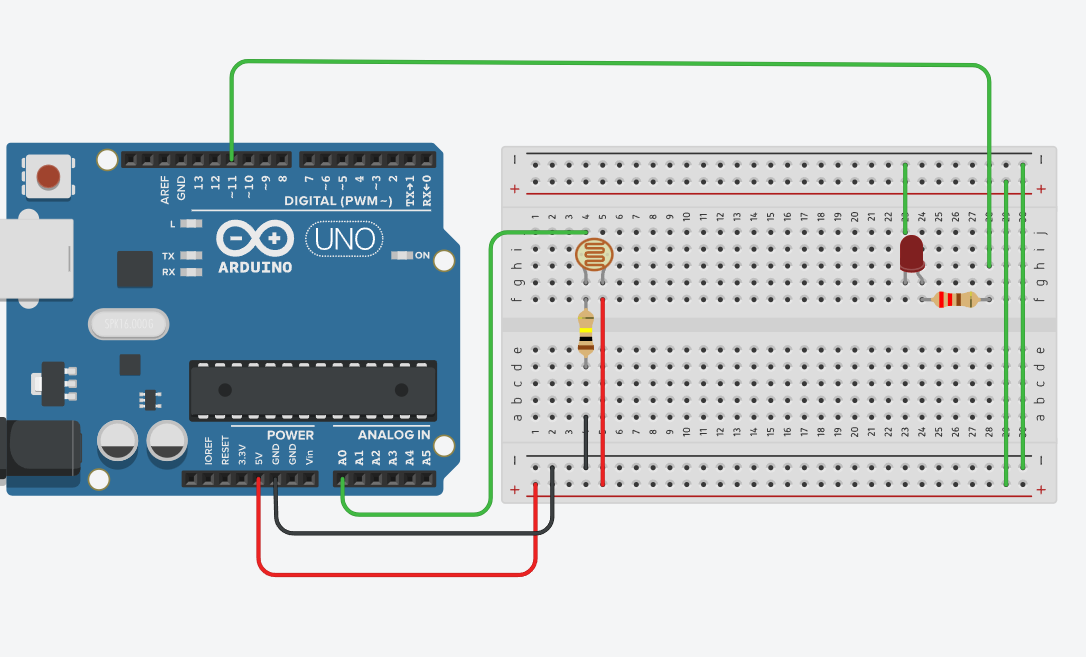
\includegraphics[width=17cm]{z3/1.png}
	\caption{схема сборки}
\end{figure}
\begin{figure}[H]
	\centering
	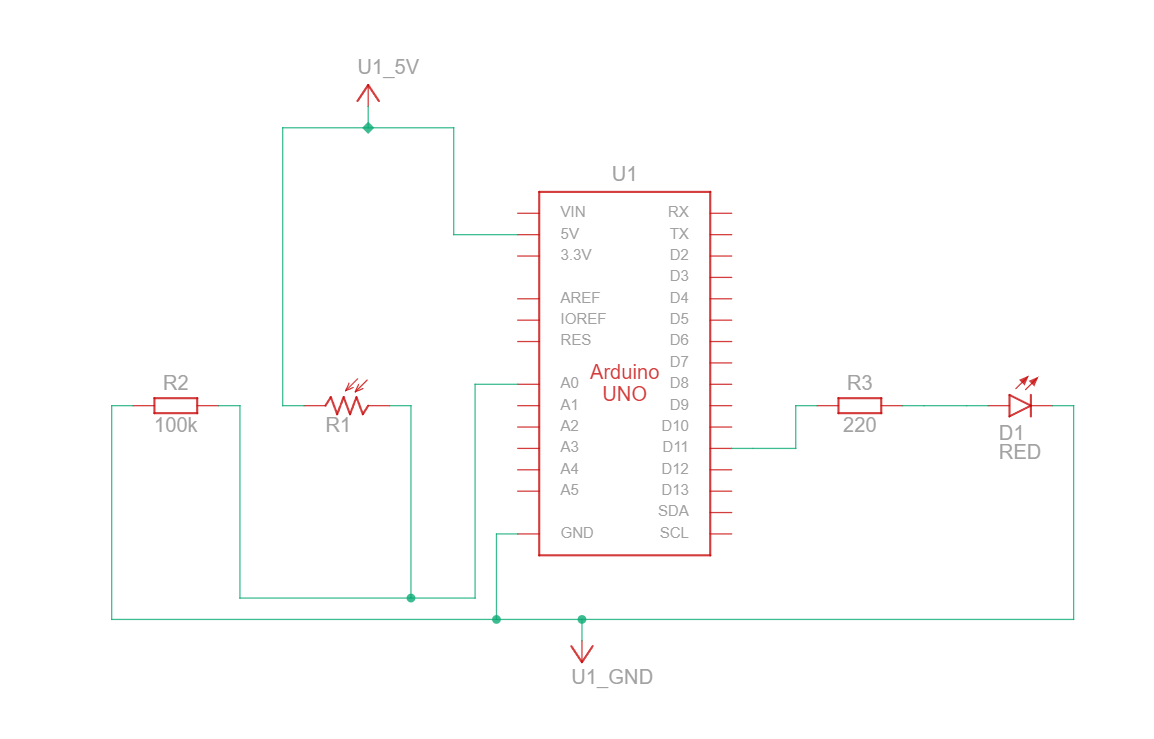
\includegraphics[width=17cm]{z3/2.png}
	\caption{принципиальная схема}
\end{figure}
Код прошивки:
\inputminted{cpp}{z3/main.cpp}
Получаемый с пина A0 сигнал от фоторезистора в аудитори в среднем имеет значение 890-910, при полном закрытии он выдаёт 160-350, а при свете фонарика он максымум выдаст 1000-1010. Для максимальной и минимальной яркости светодиода используется вычетание и проверки значения с датчика.
https://www.tinkercad.com/things/aPxT8gU4ksx-praktika-1-zadacha-3
\section{Азбука Морзе}
\begin{verbatim}
	Кнопка: Срабатывание по отжатию
\end{verbatim}
\begin{figure}[H]
	\centering
	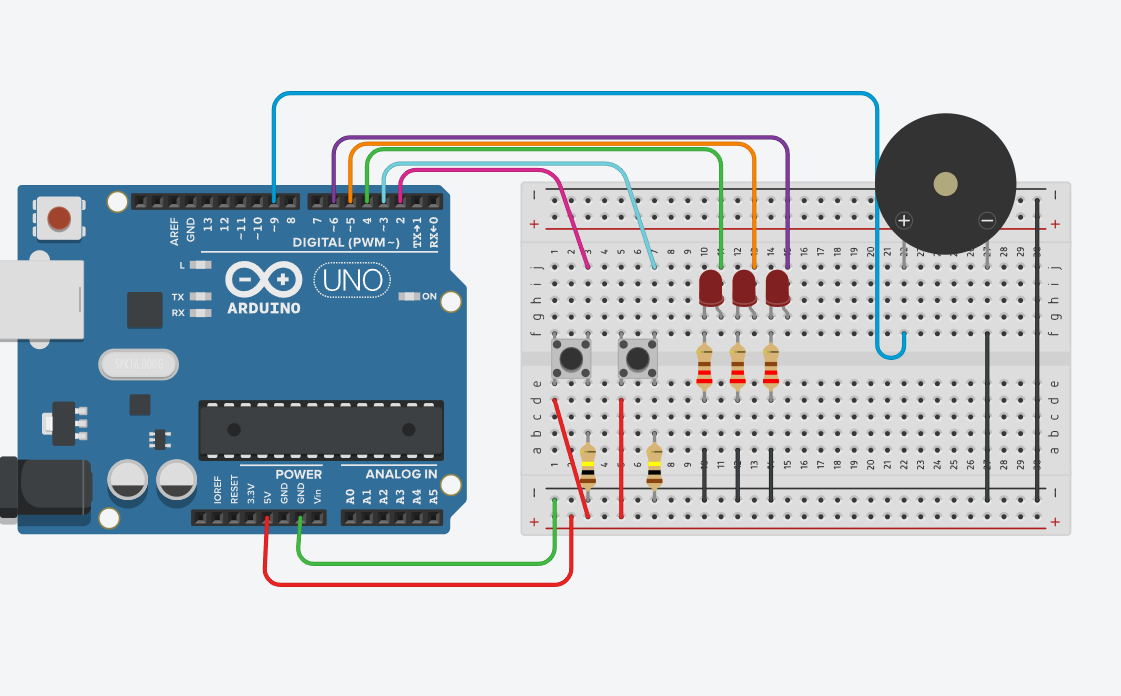
\includegraphics[width=17cm]{z4/1.png}
	\caption{схема сборки}
\end{figure}
\begin{figure}[H]
	\centering
	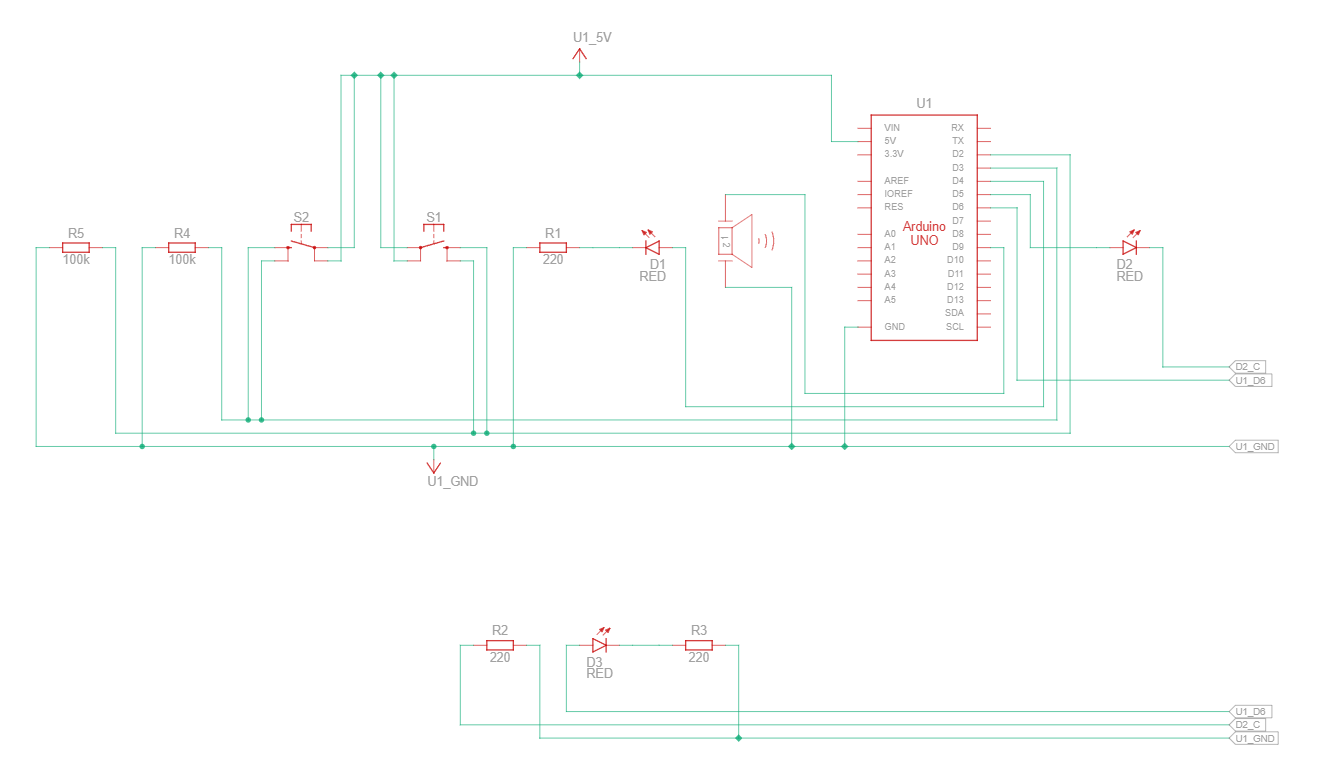
\includegraphics[width=17cm]{z4/2.png}
	\caption{принципиальная схема}
\end{figure}
Код прошивки:
\inputminted{cpp}{z4/main.cpp}
Первая кнопка переключает мелодию, вторая останавливает текущую мелодию. Флаги "first\_selected"\ и "running"\ отвечают за выбор и воспроизведение мелодии соответсвенно. В зависимости от выбранной мелодии загорается первый или второй светодиод, а также третий светодиод мигает когда звучит не нулевая частота.
https://www.tinkercad.com/things/088R8NWJdHL-muzon
\section{Терменвокс}
\begin{verbatim}
	При падении освещенности звук: Увеличивается
	Звуковой сигнал: Непрерывно
	Частоты нот: Первая октава
\end{verbatim}
\begin{figure}[H]
	\centering
	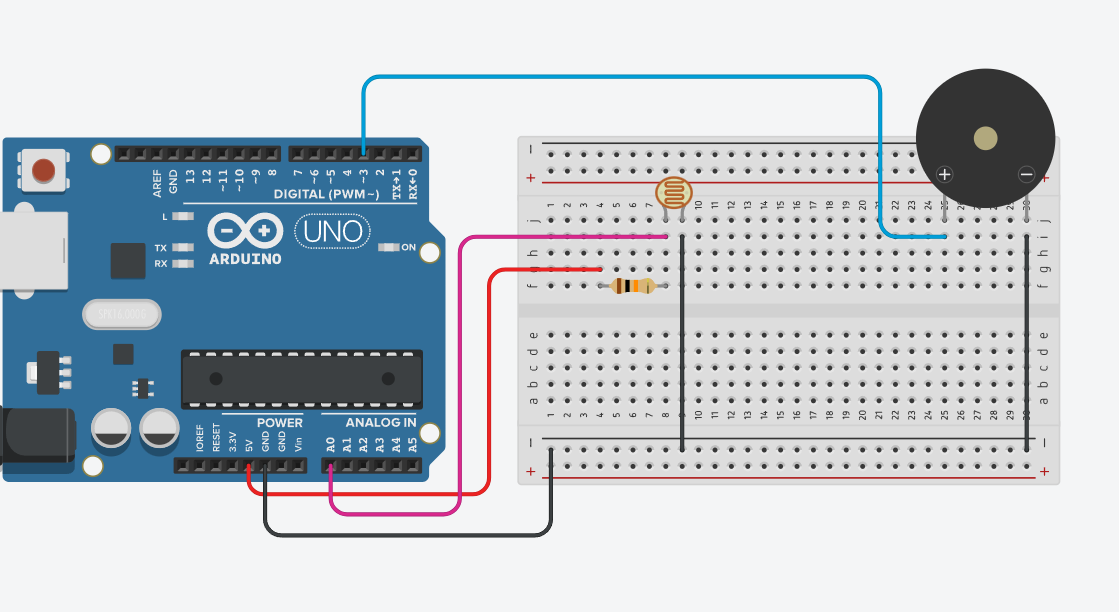
\includegraphics[width=17cm]{z5/1.png}
	\caption{схема сборки}
\end{figure}
\begin{figure}[H]
	\centering
	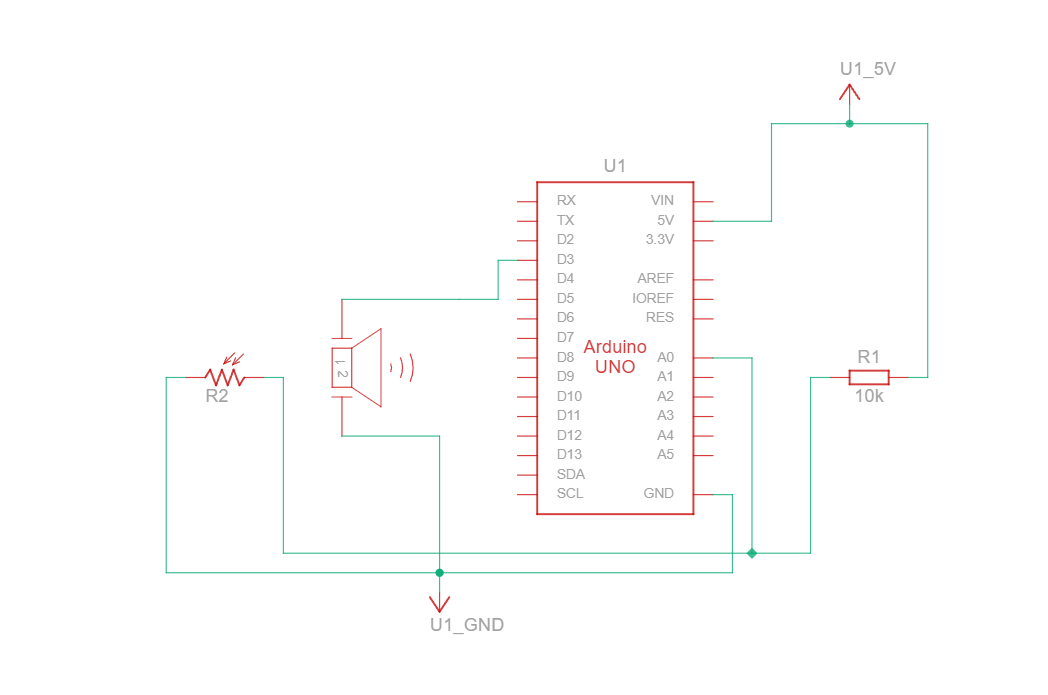
\includegraphics[width=17cm]{z5/2.png}
	\caption{принципиальная схема}
\end{figure}
Код прошивки:
\inputminted{cpp}{z5/main.cpp}
"frequency"\ хранит частоту, которую мы получаем с термистора путём преобразования его диапазона в диапазон частот Первой октавы. На термисторе выбран диапазон 400 - 500 т.к. в аудитории он остывает и стремится к 500, а при нагреве пальцами стремится к 400.
https://www.tinkercad.com/things/0ufMNffx19a-praktika-1-zadacha-5
\section{Мерзкое пианино}
\begin{verbatim}
	Подключение кнопок: Стягивающий резистор
	Входной сигнал: switch/case
	Частоты нот: Вторая октава
\end{verbatim}
\begin{figure}[H]
	\centering
	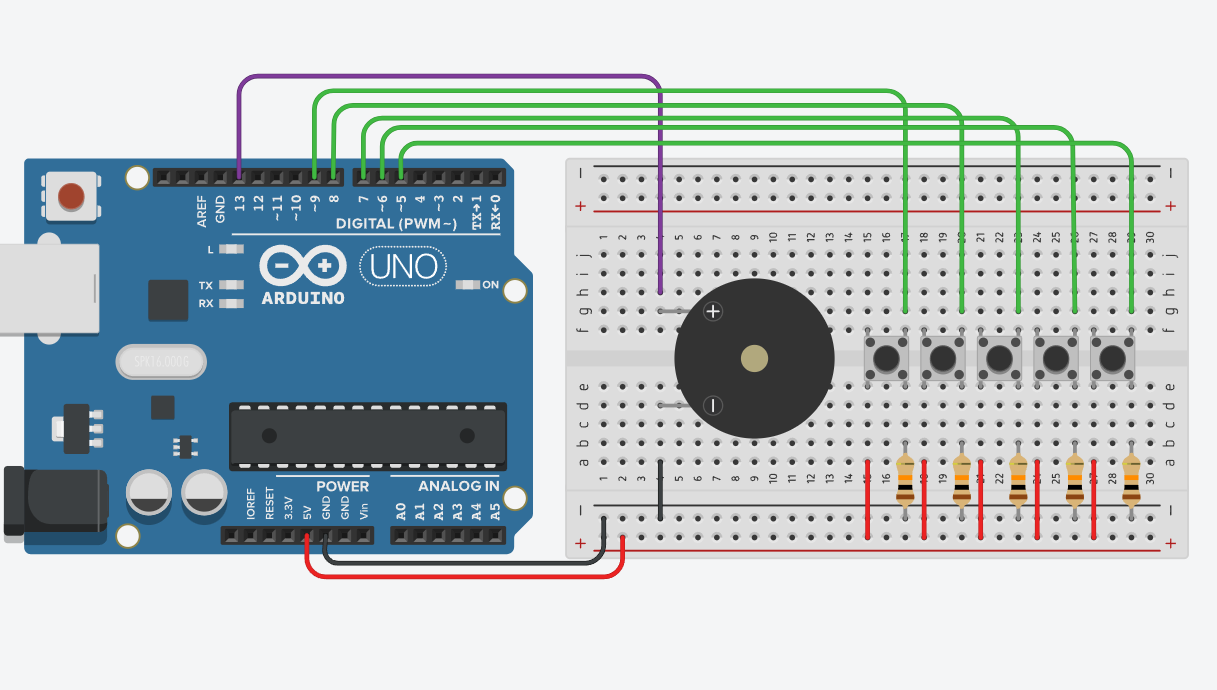
\includegraphics[width=17cm]{z6/1.png}
	\caption{схема сборки}
\end{figure}
\begin{figure}[H]
	\centering
	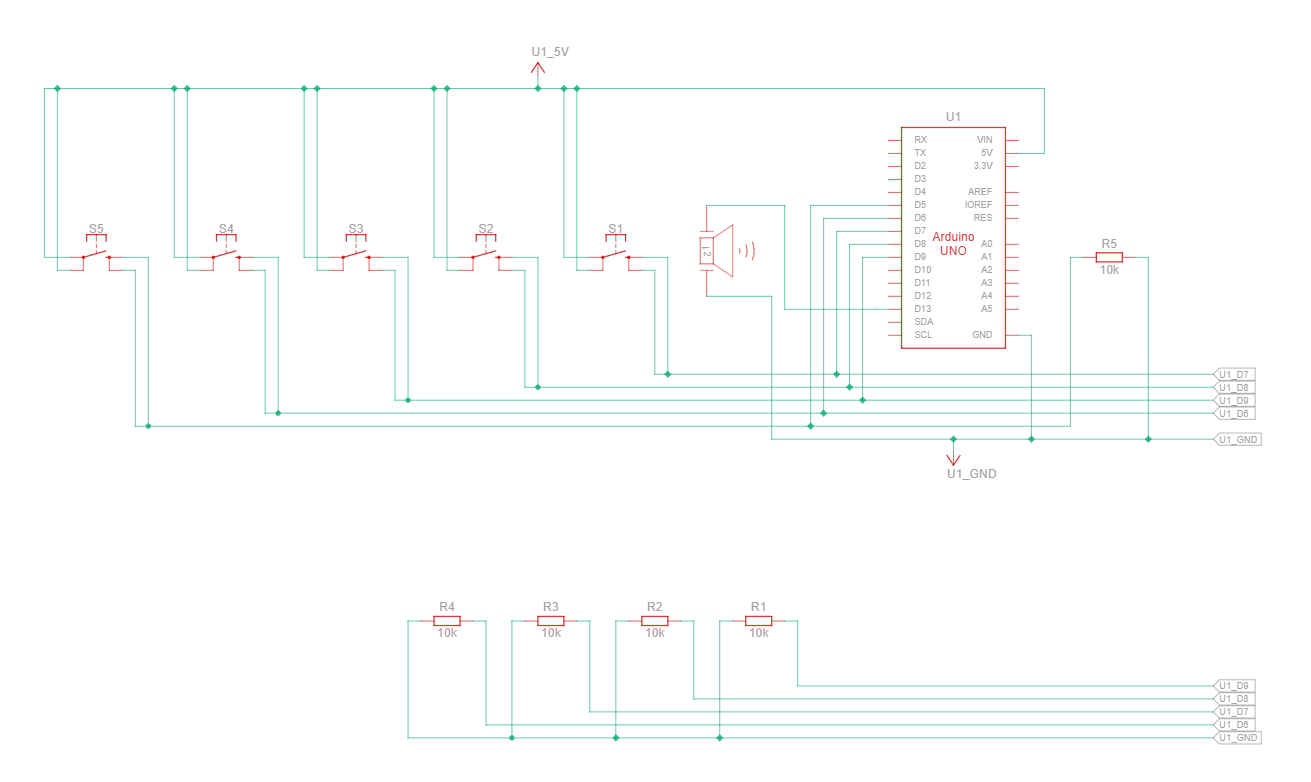
\includegraphics[width=17cm]{z6/2.png}
	\caption{принципиальная схема}
\end{figure}
Код прошивки:
\inputminted{cpp}{z6/main.cpp}
"index"\ - как указатель в цикле, проходит по значениям от 0 до 4. в "b"\ хранятся предыдущие состояния кнопок нажата/не нажата, а в "m"\ хранятся частоты. в "btn"\ записывается текщее состояние текущей кнопки и сравнивается с предыдущим её состоянием.
https://www.tinkercad.com/things/2iVt3yc7YIU-praktika-1-zadacha-6